\documentclass[12 pt., oneside, letterpaper]{article}
\usepackage{hyperref}
\usepackage[utf8]{inputenc}
\usepackage{graphicx}
\usepackage{booktabs}
\usepackage{datatool}
\graphicspath{ {./graph/}}
\hypersetup{
    colorlinks=true,
    linkcolor=blue}

\begin{center}
\title{\HUGE Analysis of Arkansas Yearly Tornado Numbers}
\author{\Large Carol Stover}
\maketitle


\end{center}


\begin{document}
\hrule{\textwidth}
\begin{abstract}
    \noindent The Southwest Times Record has an archive of data concerning tornadoes that struck Arkansas throughout the past century. This project pulled the raw data from those archives, formatted it as a text file, and plotted it in a line graph in python. This plot shows a gradual but noticeable increase in the frequency of tornadoes as the data gets more recent. This supports the idea that natural disasters have and will continue to become more common as climate change grows in intensity.  
\end{abstract}
\hrule{\textwidth}


\section{Introduction}

As climates across that world change more and more rapdily, the occurrence of natural disasters appears to have increase significantly. For residents of the southern United States,
this has meant a particularly rough 2023 tornado season. In the wake of the historic tornado that tore through Central Arkansas, it seemed like a good time to take another look at Arkansas' history with
tornadoes. The Southwest Times Record has kept a record of the number of the number of tornadoes to hit the state of Arkansas each year, all the way from 1950 to the present. For this project, I only included the information from 1950 to 2022 as the information available for 2023 is incomplete and would throw off any pattern that may be there. 
 



\section{Data}
Below is the raw data that I found on the website for the Southwest Times Record.

\input{data.txt}

 
\newpage

\section{Visualization}
\begin{center}
\begin{figure}[h]
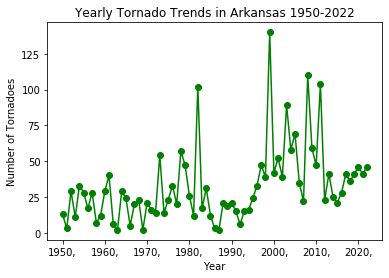
\includegraphics[width=1.0\textwidth]{graph}
\caption{A line graph showing the trend of tornadoes that occurred every year from 1950 to 2022 in Arkansas. 
         According to the graph, while there are outliers, there is a slight upward trend, suggesting the rate of tornadoes in the state has increased through the years.\cite{record_tornadoes}}
\label{fig:graph}
\end{figure}
\end{center}

\section{Results}
From \ref{fig:graph} you can see a gradual upward trend. Of course, there are some outliers, but for the most part all of the points hover around a consistent upward trend. As unpleasant as this tornado season has been, that means it's probably only going to get worse in upcoming decades. \\


\bibliographystyle{plain}
\bibliography{projectrefs.bib}

\end{document}
